\documentclass[14pt]{book}
\usepackage{array}
\usepackage{amsmath}
\usepackage{amsfonts}
\usepackage{math}
\usepackage{graphicx}
\usepackage{rsfs}
\usepackage{amssymb}
\usepackage{multicol}
\textwidth=31.9pc
\textheight=46.5pc
\oddsidemargin=1pc
\evensidemargin=1pc
\headsep=15pt
%\headheight=.2cm
\topmargin=.6cm
\parindent=1.7pc
\parskip=0pt


\setcounter{page}{1}
\begin{document}
%\pagestyle{fancy}
\renewcommand{\baselinestretch}{1.2}
%\lhead[\fancyplain{} \leftmark]{}
%\chead[]{}
%\rhead[]{\fancyplain{}\rightmark}
%\cfoot{}
%\headrulewidth=0pt
\markright{
%\hbox{\footnotesize\rm Statistica Sinica
%{\footnotesize\bf ??}(200?), 000-000}\hfill
}
\markboth{\hfill{\footnotesize\rm FIRSTNAME1 LASTNAME1 AND FIRSTNAME2 LASTNAME2
}\hfill}
{\hfill {\footnotesize\rm FILL IN A SHORT RUNNING TITLE} \hfill}
\renewcommand{\thefootnote}{}
$\ $\par
\fontsize{10.95}{14pt plus.8pt minus .6pt}\selectfont
\vspace{0.8pc}
\centerline{\large\bf How To Find A Better Convex Hull}
\vspace{2pt}
\centerline{\large\bf }
%\vspace{.4cm}
%\centerline{Author(s)}
%\vspace{.4cm}
%\centerline{\it Affiliation(s)}
\vspace{.55cm}
\fontsize{9}{11.5pt plus.8pt minus .6pt}\selectfont


\begin{quotation}
\noindent {\it Abstract:}
Propose a nearest neighbor NMF algorithm for Unsupervised Learning (Blind Source Separation), which relaxes the assumption we used and gives reasonable good results.  \par

\vspace{9pt}
\noindent {\it Key words and phrases:}
Unsupervised Learning,Blind source separation, convex hull
\par
\end{quotation}\par

\fontsize{10.95}{14pt plus.8pt minus .6pt}\selectfont
\setcounter{chapter}{1}
\setcounter{equation}{0} %-1
\noindent {\bf 1. Introduction}
Hyperspectral imaging is a remote sensing technology that collects 2-D images from the Earth's surface in hundreds of narrow and contiguous bands of high spectral resolution covering the visible, near-infrared, and shortwave infrared bands. The spatial resolution corresponding to a single pixel of a hyperspectral image depends on the flying height of the aircraft and on the instantaneous fields of view of the sensors. Very often, the resolution cells, in an image, contain several substances. Thus, the radiances collected in the spectral vectors are mixture of spectra from the constituent substances(also called endmembers) present in the respective resolution cells. 
\par The linear mixing assumption has been widely used to describe the observed hyper spectral vectors. According to this assumption, a mixed pixel is a linear combination of endmember signatures weighted by corresponding abundance fractions. Due to physical considerations, the abundance fractions are subject to the so-called non negativity and a full-additivity(sum-to-one) constraints. Thus, the observed spectral vectors in a given scene are in a simplex whose vertices corresponding to endmembers.

 


The model for hyper spectral imaging unmixing can be expressed as 
\begin{equation}
X = A*S+N
\end{equation}
In this report, we will focus on the non-negative components separation. 
\begin{equation}
\begin{aligned}
& X = A*S+N
& & S_{i,j}\geq 0,A_{i,j}\geq 0
\end{aligned}
\end{equation}
Here, $X$ is the observed $m$-dimensional mixture signal, each row of $X$ represents one mixture signal. $A$ is mixing matrix. $S$ represents $n$-dimensional source signals, $n<=m$, each row of $S$ represents one source signal.  $N$ represents noise(often assumed to be while Gaussian). The goal here is to recover both $A$ and $S$ given only $X$. 
This is a ill-posed problem. Different assumptions are proposed based on application fields. 
\par Two types of objective function are considered for blind source separation problem. one is 
\begin{equation}
{\text{minimize}} \parallel X-A*S \parallel ^2
\end{equation}
The other is Kullback-Leibler divergence cost function. In this report, we will focus on the first objective function.
One view to understand all these different algorithms is to look at constraints and regularizers. 
For example, one side of the spectrum of these algorithms is kmeans algorithm. 
\begin{equation}
\begin{aligned}
& \underset{S}{\text{argmin}}
& & \sum_{i=1}^k {\sum _{x_j\in S_i } {\left \| x_j-\mu_i  \right \|^2}}  \\
\end{aligned}
\end{equation}
when basis $A$ is fixed, the kmeans algorithm encoding corresponding to vector quantization. It gives strongest constraint that each column of $S$ has only 1 one and others are 0s. We can reform Kmeans by the following: 

\begin{equation}
\begin{aligned}
& \underset{A,S}{\text{min}}
& & \parallel X-A*S \parallel ^2   \\
& \text{subject to}
& & \text{each column of $S$ has only 1 one and others are 0s.}
\end{aligned}
\end{equation}
where  the columns for $A$ are $\mu_i$'s .  

\par At the other side of the spectrum for these algorithms , is Non-negative Matrix Factorization(NMF). 
\begin{equation}
\begin{aligned}
& \underset{A,S}{\text{min}}
& & \parallel X-A*S \parallel ^2   \\
& \text{subject to}
& & S_{i,j}\geq 0,A_{i,j}\geq 0
\end{aligned}
\end{equation}
\setcounter{chapter}{2}
\setcounter{equation}{0} %-1
Although the function $ \parallel X-A*S \parallel ^2 $ are convex in $A$ only or $S$ only, they are not convex in both variables together. Therefore it is unrealistic to expect an algorithm to solve this problem in the sense of finding a global minima. However, there are many techniques from numerical optimization that can be applied to find local minima.
When we use the following update rule, $S$ and $A$ will converge to a local minimum. Gradient descent is perhaps the simplest technique to implement, but convergence can be slow. Other methods such as conjugate gradient have faster convergence, at least in the vicinity of local minima, but are more complicated to implement than gradient descent.The convergence of gradient based methods also have the disadvantage of being very sensitive to the choice of step size, which can be very inconvenient for large applications. One updates rules are the following:

\begin{equation}
\begin{aligned}
& S_{\alpha \mu }\leftarrow S_{\alpha \mu }\frac{(A^{T}X)_{\alpha \mu }}{(A^{T}AX)_{\alpha \mu }} \\
& A_{\beta \alpha }\leftarrow A_{\beta \alpha }\frac{(XS^{T})_{\beta \alpha }}{(ASS^{T})_{\beta \alpha }} 
\end{aligned}
\end{equation}
This is proved to converge. 


In the middle of the spectrum, we have the algorithm proposed by Naanaa, I call it self-convex-hull algorithm. 
\begin{equation}
\begin{aligned}
& \underset{A,S}{\text{min}}
& & \parallel X-A*S \parallel ^2   \\
& \text{subject to}
& & S_{i,j}\geq 0,A_{i,j}\geq 0 \\
& \text{and}
& & \text{S has columns of} \begin{bmatrix}
1\\ 
0\\ 
0\\ 
0
\end{bmatrix}
& & \begin{bmatrix}
0\\ 
1\\ 
0\\ 
0
\end{bmatrix}
& & \begin{bmatrix}
0\\ 
0\\ 
1\\ 
0
\end{bmatrix}
& & \begin{bmatrix}
0\\ 
0\\ 
0\\ 
1
\end{bmatrix}
\end{aligned}
\end{equation}
The way to compute $A$ and $S$ under this assumption is quite simple. Notice that the set of all the columns of mixing matrix $A$ are a subset of  the columns of $X$. Naanaa proposed the following algorithm. 

1. Discard from $X$ those columns $X^j$ such that $\left \| X_{j} \right \|\leq \varepsilon$ Note $X$ the resulting matrix. 
\par 2. Form the matrix $X$ consisting of all the mutually nonlinear columns of $X$. 
\par 3. For each column $X^j$ $(j=1, \ldots, m.)$, solve the optimization problem: 
\begin{equation}
\begin{aligned}
& \underset{}{\text{minimize}}
&  \left \| X^{\o j}\alpha(j)-X^j \right \|,   \\
& \text{subject to}
&  \alpha_i(j)\geq 0 (j=1, \ldots, m.)\\
\end{aligned}
\end{equation}
and compute score for $X^j$ 
\begin{equation}
\begin{aligned}
score_j = \left \| X^{\o j}\alpha(j)-X^j \right \|
\end{aligned}
\end{equation}
\par 4. Select the $n$ columns of $X$ which are associated with the highest score and form matrix $A$


We can see that, comparing with Kmeans, instead of requiring all the columns have only $1$ one and others are $0$s, this algorithm only require existing the columns of 
\begin{equation}
\begin{aligned}
& &\begin{bmatrix}
1\\ 
0\\ 
0\\ 
0
\end{bmatrix}
& & \begin{bmatrix}
0\\ 
1\\ 
0\\ 
0
\end{bmatrix}
& & \begin{bmatrix}
0\\ 
0\\ 
1\\ 
0
\end{bmatrix}
& & \begin{bmatrix}
0\\ 
0\\ 
0\\ 
1
\end{bmatrix}
\end{aligned}
\end{equation}
In this report , my goal is to relax the constraint even more. In real data, e.g. time series data, we might not be able to find a time point that all other source signals totally disappear except one.  But we might find several time points that only one signal is dominated . Mathematically speaking, my assumption is that there existing columns of 
\begin{equation}
\begin{aligned}
& &\begin{bmatrix}
1\\ 
\epsilon_1\\ 
\epsilon_2\\ 
\epsilon_3
\end{bmatrix}
& & \begin{bmatrix}
\epsilon_1\\ 
1\\ 
\epsilon_2\\ 
\epsilon_3
\end{bmatrix}
& & \begin{bmatrix}
\epsilon_1\\ 
\epsilon_2\\ 
1\\ 
\epsilon_3
\end{bmatrix}
& & \begin{bmatrix}
\epsilon_1\\ 
\epsilon_2\\ 
\epsilon_3\\ 
1
\end{bmatrix}
\end{aligned}
\end{equation}
\setcounter{chapter}{2}
\setcounter{equation}{0} %-1



{\bf 2. Motivation}
An important observation is that, geometrically thinking, we can consider the column vectors of matrix $A$ as the support vectors for a convex hull. All the column vectors of $X$ are our observed data points that are in such convex hull. Let $A_i$ represents the columns of matrix $A$, or geometrically speaking, the support vectors. $X_j$ are the column vectors of $X$, or geometrically speaking , the data vectors we can observe .The BSS problem is how to find the correct support vectors for the observed data points. To comparing all these algorithms, we would like to represent them in such geometric point of view. The  Kmeans algorithm is saying all the column vectors of are actually support vector themselves. No point is actually inside the convex hull. The NMF algorithm is make sure all the data vectors  $X_j$ are in such convex hull, but put no constraints on where these support vectors $A_i$ are. The self-convex-hull algorithm is saying the support vectors $A_i$ are a subset of the data vectors of $X_j$s. It means we pick the best support vectors from the given data vectors. Under my assumption that there existing columns of 
\begin{equation}
\begin{aligned}
& &\begin{bmatrix}
1\\ 
\epsilon_1\\ 
\epsilon_2\\ 
\epsilon_3
\end{bmatrix}
& & \begin{bmatrix}
\epsilon_1\\ 
1\\ 
\epsilon_2\\ 
\epsilon_3
\end{bmatrix}
& & \begin{bmatrix}
\epsilon_1\\ 
\epsilon_2\\ 
1\\ 
\epsilon_3
\end{bmatrix}
& & \begin{bmatrix}
\epsilon_1\\ 
\epsilon_2\\ 
\epsilon_3\\ 
1
\end{bmatrix}
\end{aligned}
\end{equation}
I would like the support vector to form a slightly bigger convex hull, comparing with self-convex-hull algorithm. 
\par Come back to the optimization point of view again.Again, let $A_i$ represents the columns of matrix $A$, or geometrically speaking, the support vectors. $X_j$ are the column vectors of $X$, or geometrically speaking , the data vectors we can observe . $XN_{i1}$ is the corresponding nearest neighbor point of $A_i$ in the data vectors set. For self-convex-hull algorithm, since the support vectors are picked from the data vectors, which means the following optimization algorithm
\begin{equation}
\begin{aligned}
& \underset{A,S}{\text{min}}
& & \parallel X-A*S \parallel ^2 + \lambda \parallel A_i-XN_{i1} \parallel^2  \\
& \text{subject to}
& & S_{i,j}\geq 0,A_{i,j}\geq 0, \lambda = +\infty\\
\end{aligned}
\end{equation}
$\lambda = +\infty$ here to force the support vector to be chosen from the data vector sets. 
\setcounter{chapter}{3}
\setcounter{equation}{0} %-1

{\bf 3. Our Approach}
 Look at the optimization (2.2), comparing with my assumption that 
 there existing several columns of 
\begin{equation}
\begin{aligned}
& &\begin{bmatrix}
1\\ 
\epsilon_1\\ 
\epsilon_2\\ 
\epsilon_3
\end{bmatrix}
& & \begin{bmatrix}
\epsilon_1\\ 
1\\ 
\epsilon_2\\ 
\epsilon_3
\end{bmatrix}
& & \begin{bmatrix}
\epsilon_1\\ 
\epsilon_2\\ 
1\\ 
\epsilon_3
\end{bmatrix}
& & \begin{bmatrix}
\epsilon_1\\ 
\epsilon_2\\ 
\epsilon_3\\ 
1
\end{bmatrix}
\end{aligned}
\end{equation}
I came out of two ideas. The key here is notice that the assumption means several data vector points will locate near the support vectors. So we should  penalize the distance from the support vector to its k-nearest neighbor points, which gives  the following optimization problem
\begin{equation}
\begin{aligned}
& \underset{A,S}{\text{min}}
& & \parallel X-A*S \parallel ^2 + \lambda \parallel A_i-1/K*(XN_{i1}+XN_{i1}+ \ldots +XN_{iK}) \parallel^2  \\
& \text{subject to}
& & S_{i,j}\geq 0,A_{i,j}\geq 0, \lambda \geq 0
\end{aligned}
\end{equation}
$\lambda$ here is not +$\infty$ but a positive parameter, adjusting how large I want the convex hull to be.  
When $\lambda$ gets bigger, the convex hull gets smaller.
Applying alternative direction method,we can optimize by alternating the following steps 

Fixed $S$, update $A$ \\
1.$A = ((SS^T)^{-1}SX^T)^T$\\
2.$A_i = A_i - \lambda*(A_i-1/K*(XN_{i1}+XN_{i1}+ \ldots +XN_{iK}))$\\
3.project all negative element of $A$ to $0$.\\
\par Fixed $A$, update $S$ \\ 
1.$S =(A(A^TA)^{-1})^TX$\\
2.project all negative elements of $S$ to $0$.


\setcounter{chapter}{4}
\setcounter{equation}{0} %-1
\noindent {\bf 4. Data Set and Experiment Results }
At this stage , I only use synthetic data to evaluate the performance of the algorithm.  
3 source signals are considered here, since we can view the convex hull  in dimension 3. 

\setcounter{chapter}{5}
\setcounter{equation}{0} %-1
\noindent {\bf 4. Future Work}
\begin{figure}[ht!]

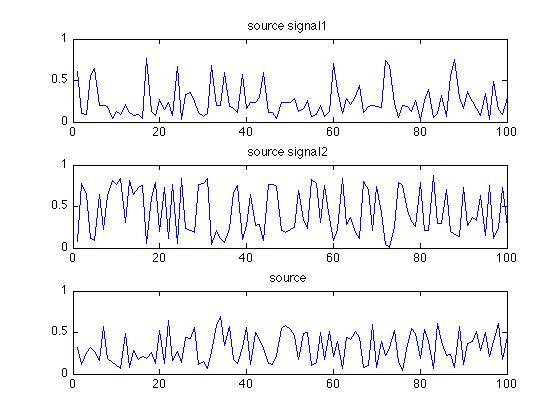
\includegraphics[width=150mm,height = 50mm]{eg1source.jpg}
\caption{e.g.1 Source Signals}
\label{overflow}
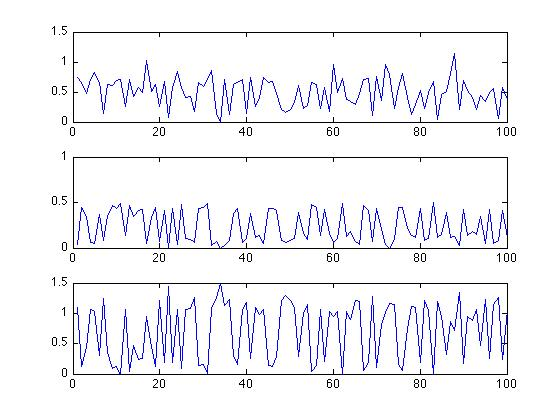
\includegraphics[width=150mm,height = 50mm]{eg1recoveredByNMF.jpg}
\caption{e.g.1 Recovered By NMF Signals}
\label{overflow}
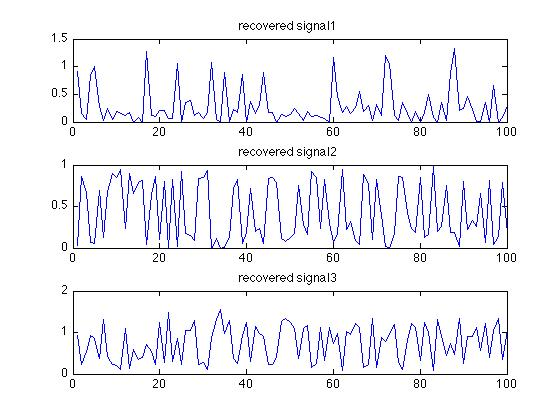
\includegraphics[width=150mm,height = 50mm]{eg1RecoveredByNewAlgorithm.jpg}
\caption{e.g.1 Recovered By New Algorithm Signals}
\label{overflow}
\end{figure}

\par
\begin{figure}[ht!]

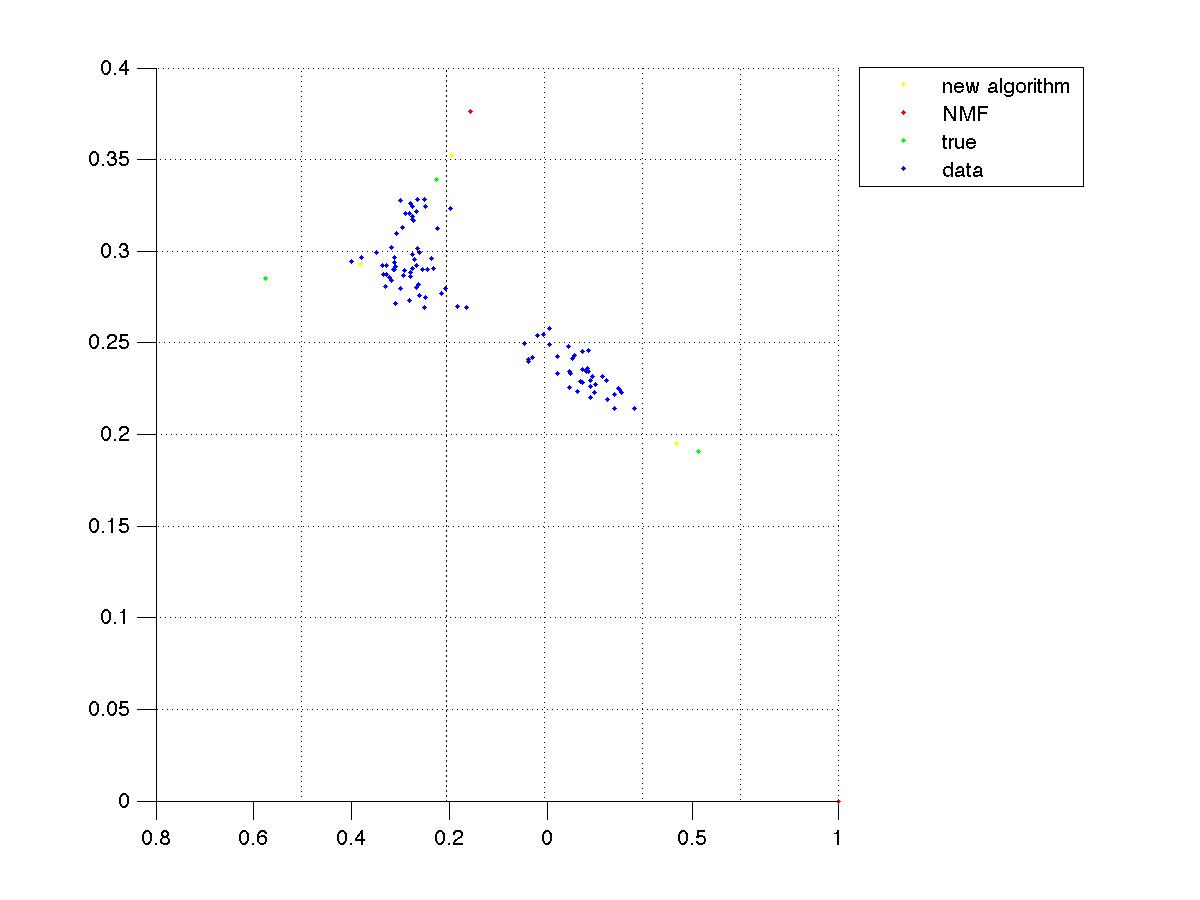
\includegraphics[width=150mm,height = 120mm]{eg1.jpg}
\caption{e.g.1 data vectors and support vectors visualization }
\label{overflow}
\end{figure}

\begin{figure}[ht!]

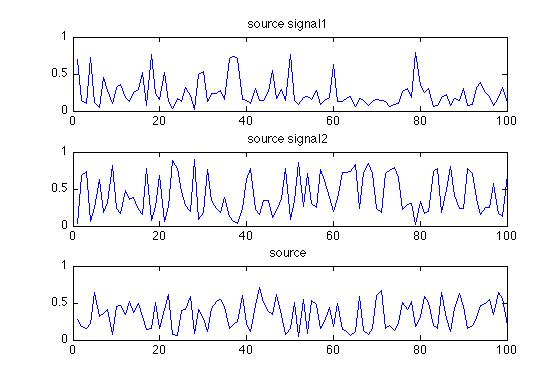
\includegraphics[width=150mm,height = 50mm]{eg2s.jpg}
\caption{e.g.2 Source Signals}
\label{overflow}
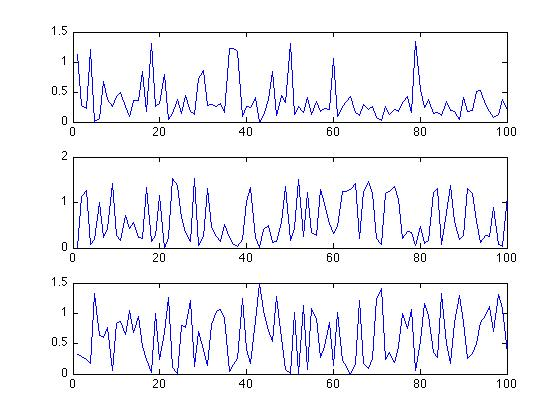
\includegraphics[width=150mm,height = 50mm]{eg2NMF.jpg}
\caption{e.g.2 Recovered By NMF Signals}
\label{overflow}
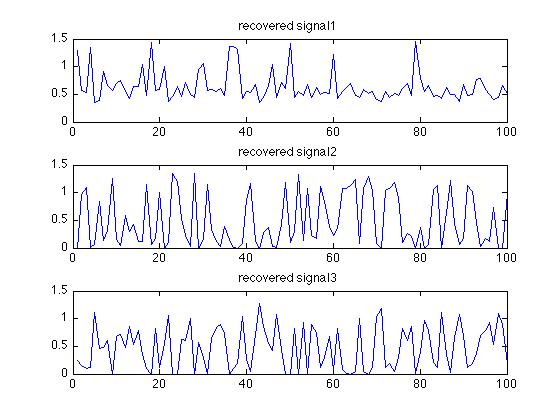
\includegraphics[width=150mm,height = 50mm]{eg2new.jpg}
\caption{e.g.2 Recovered By New Algorithm Signals}
\label{overflow}
\end{figure}

\par
\begin{figure}[ht!]

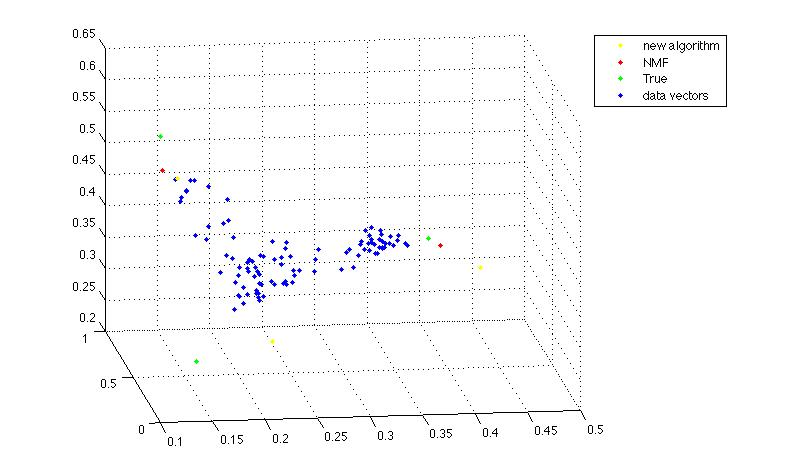
\includegraphics[width=150mm,height = 120mm]{eg2.jpg}
\caption{e.g.2 data vectors and support vectors visualization }
\label{overflow}
\end{figure}

\par

\setcounter{chapter}{5}
\setcounter{equation}{0} %-1
\begin{thebibliography} {99}
\end{thebibliography}
\vskip .65cm
\noindent
first author affiliation
\vskip 2pt
\noindent
E-mail: (first author email)
\vskip 2pt
\noindent
second author affiliation
\vskip 2pt
\noindent
E-mail: (second author email)
\vskip .3cm
%\centerline{(Received xxx 200?; accepted xxx 200?)}\par
\end{document}
